\chapter{Web Application}\label{chap:web_app}

In this section, we will describe the proposed web application for novel song recommendation which we called the \textit{SongRecommender}. The section is structured as follows: 
\begin{itemize}
    \item In Section \ref{sec:analysis} we analyze our application goals and describe what the user can expect from our application.
    \item In Section \ref{sec:implementation} We briefly introduce the building blocks of our application with focus on the individual similarity measures implementation and calculation of recommendations.
    \item In Section \ref{sec:configurations} We present the possible configurations of our application.
\end{itemize}

 The source code of this project is included in Attachment \ref{attach:first_attachment} together with user documentation which we decided not to include in this thesis. The modules we are referring to in this chapter can also be found there. To navigate the various modules and directories, see \texttt{README.md} which can be found in the attachment in the \texttt{songRecommender\_project} directory.
 
\section{Analysis}\label{sec:analysis}

There exist many music recommendation apps on the web such as YouTube\footnote{www.youtube.com}, Spotify\footnote{www.spotify.com} etc. They have a lot of data about users, user activity, a lot of songs, a lot of tags. Our application does not aspire on growing to such extend. We want to provide our users with an inspiration for new songs which they can then play on another musical platform (for example on YouTube or Spotify). 

We aim to provide common web app functionalities such as creating accounts, logging in and out, browsing individual songs, etc. Besides that, since it is a song recommender application, we also want to propose recommendations to users, let them create playlists, search for songs and like and dislike songs to improve the suggestions. Moreover, we want the users to be able to add songs they already know and that are missing in the application in order to explore which songs are similar to it based on various recommendation methods. We are also aiming on providing information about the application and its similarity measures, so even if the recommendations do not seem relevant to the user, it might be interesting for him to see, which songs are similar to which based on, for example, lyrics. It is an opportunity for a more hands on experience and it makes it not only about music but also a bit about the theory behind this application. 

\section{Implementation}\label{sec:implementation}
In this section, we present the overall architecture of our application with focus on the recommendation functionalities which are described in more detail in Subsection \ref{ssec:measure_implementation}. 

\subsection{Technologies}

We build our web application in the Django\footnote{https://www.djangoproject.com} framework using Python 3.6. We chose Python\footnote{https://www.python.org} because it is well suited for machine learning and Django because it is a Python based framework. To ensure a smooth user experience while performing complex computational tasks, we included Celery\footnote{http://www.celeryproject.org}, an asynchronous task queue, to run expensive tasks in the background. We used RabbitMQ\footnote{https://www.rabbitmq.com} as Celery's message broker. We chose the PostgreSQL\footnote{https://www.postgresql.org} database to store the data instead of Django's default --- SQLite --- because it provides support for \texttt{ArrayFields} which are an efficient and convenient way of storing the calculated song's feature vectors.

\subsection{Design}
The application follows the Model-Template-View (MTV) pattern which is a variation of the standard Model-View-Controller (MVC) pattern with the difference that the Django framework handles the controller part itself. The controller part would in this case be the processes that send the requests to the appropriate view according to the url configuration.
This pattern is pre-wired in Django.

The \textit{model} part handles the data representation as it does in the MVC pattern. The main things we need to store are the songs with their attributes such as title, artist, etc. and the representations of the implemented methods. We also need to store the users, lists that users create and similarities which we use to calculate recommendations.

The \textit{template} part is an analogy to the view part in MVC and handles how the data is displayed to the user in the form of HTML5 templates.

The \textit{view} handles what data is displayed to the user so it does a part of the job of the view from MVC. It also contains the business logic of the application so one could say that it is also a variation of the controller or rather a bridge between the models and templates and the Django controller. In the songRecommender application, the views call functions from the "logic" part of the application which takes care of calculating recommendations.


\subsubsection{Models and Database}
For every table in the database, there is a class-based model in the module \texttt{models.py} specifying its features. There is a class of the same name for the \texttt{Song} and the \texttt{List} tables. The \texttt{Profile} model which is an extension of the build-in Django \texttt{User} model is included to enable storing the similarities of songs to the user and also checking if the user has confirmed his email.
 
The class \texttt{Song\_in\_list} keeps track of songs and lists that belong to each other, an instance of the \texttt{Played\_song} model specifies a user and a song he has played. One cannot un-play a song but it can be disliked and it will not appear anymore in recommendations and it will also not be used to calculate recommendations of other songs. 

There are three different models for storing similarities. As mentioned in Chapter \ref{chap:experiments} even though we calculate and store similarities between songs they are named as if it were distances. The models are called \texttt{Distance} whose instances store basic similarities between two songs, \texttt{Distance\_to\_list} whose instance stores a similarity of a song to a particular list and \texttt{Distance\_to\_user} whose instance stores the similarity of a song to a particular user. 
\begin{figure}[ht]
    \centering
	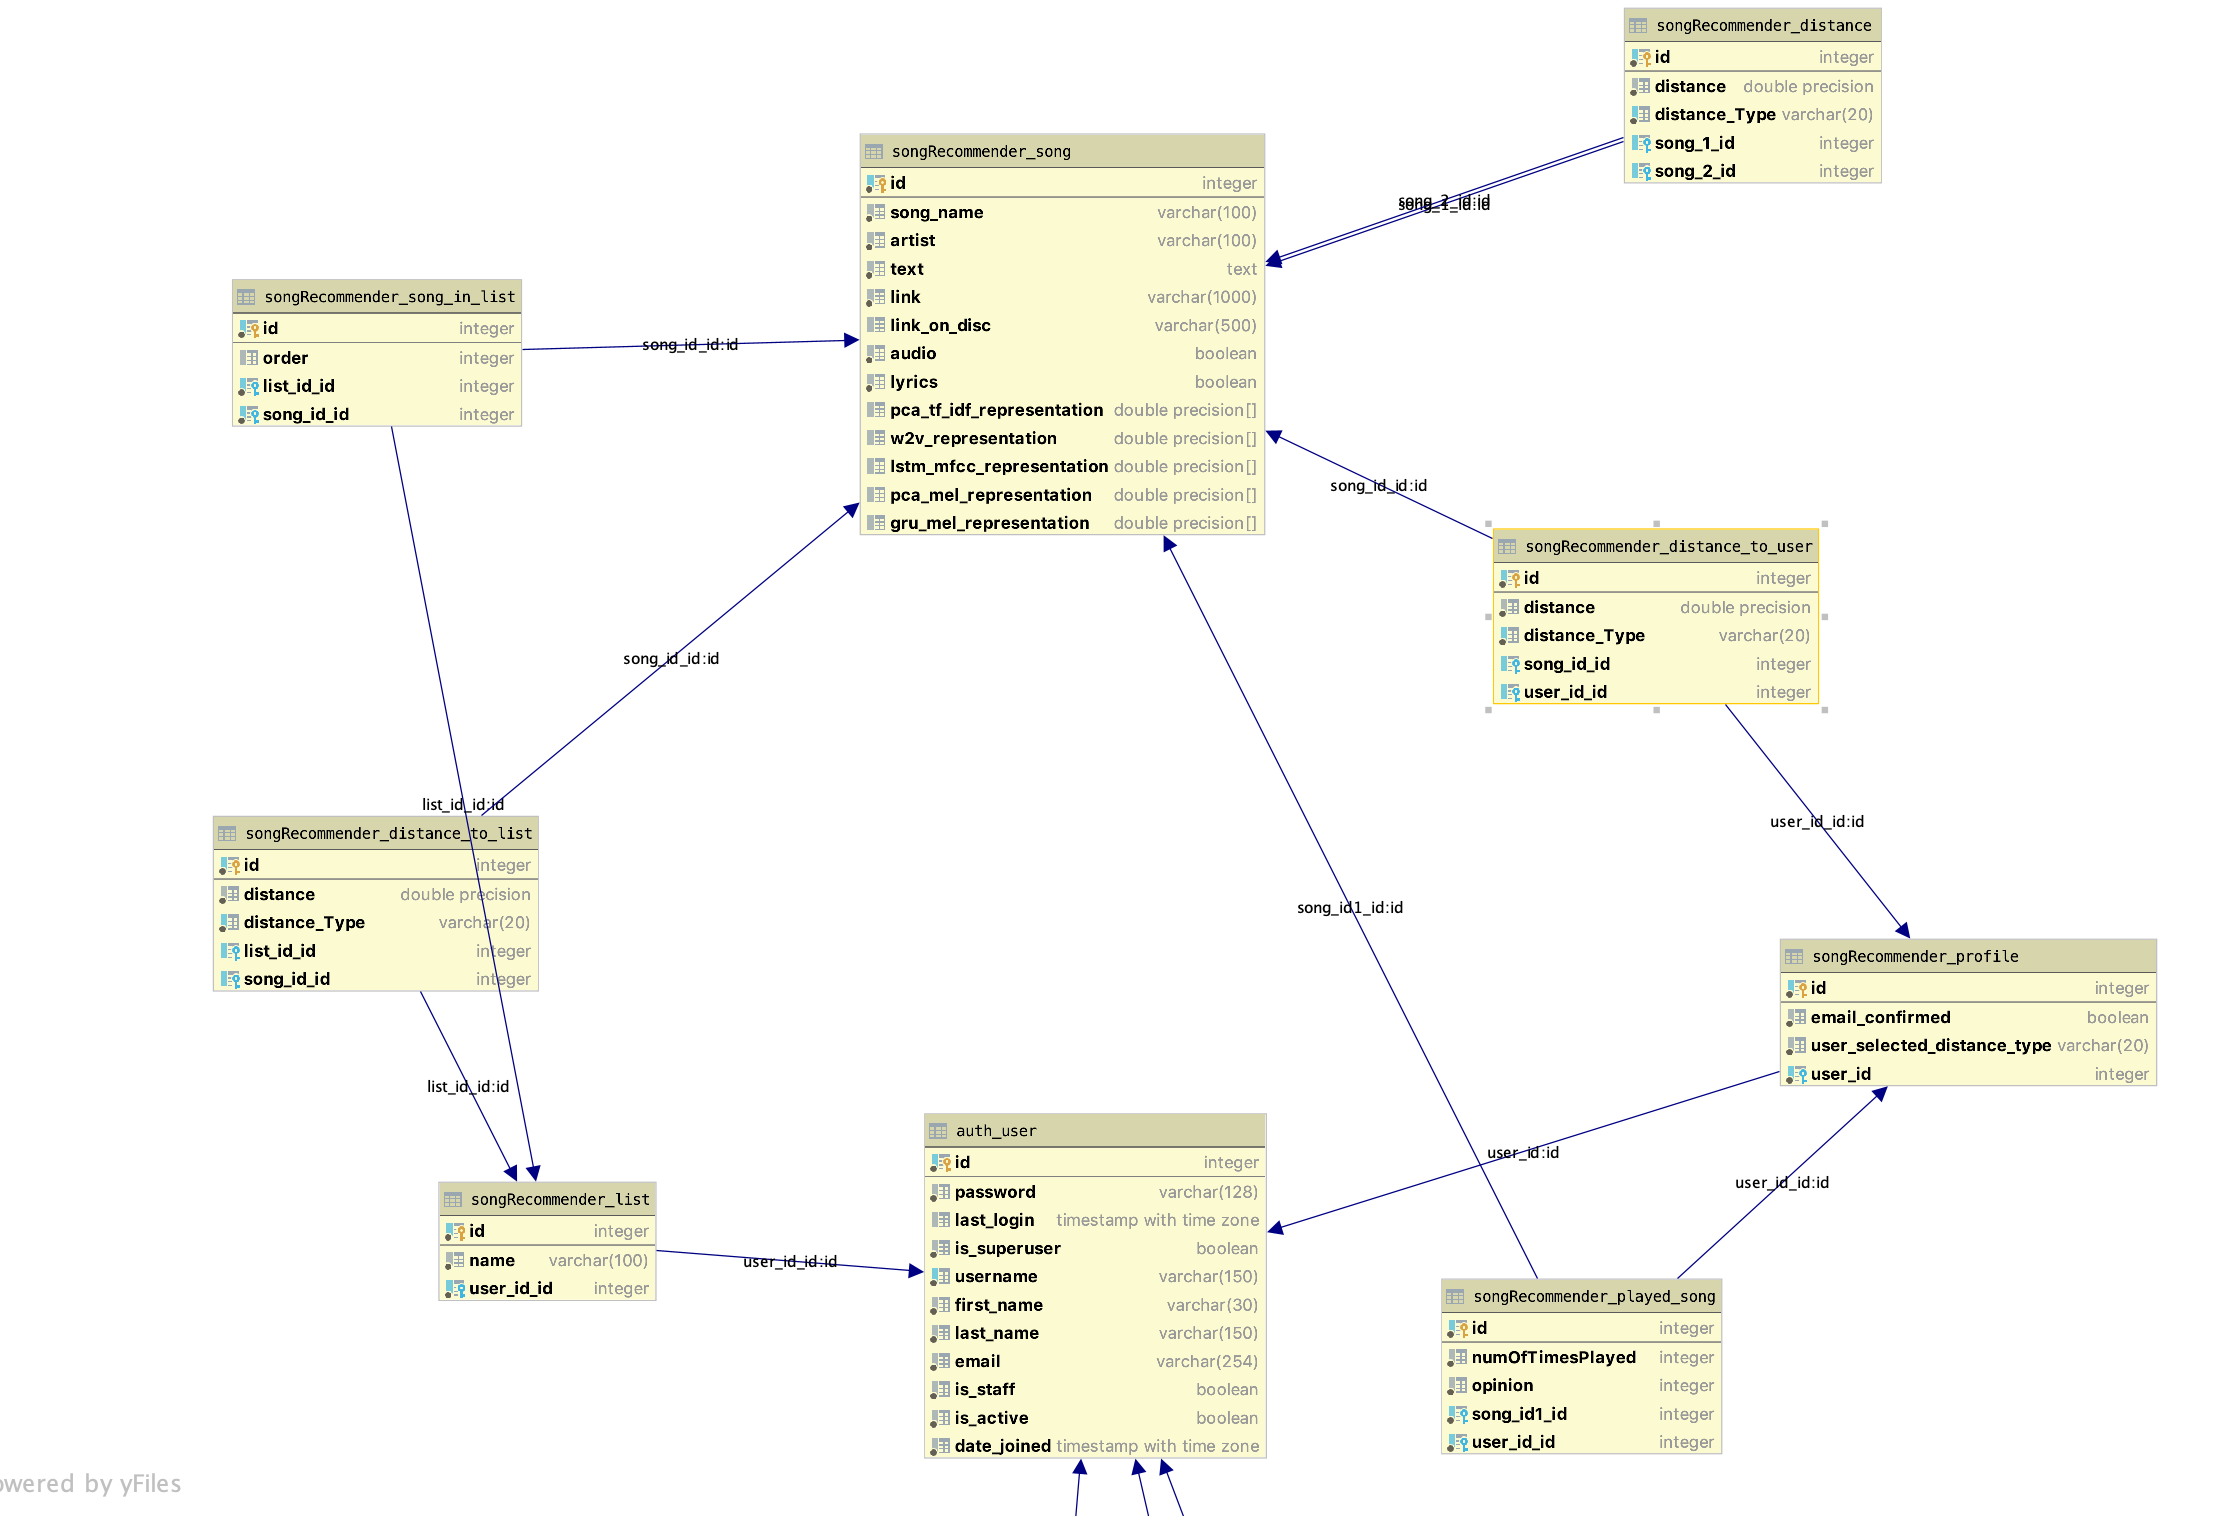
\includegraphics[width=120mm]{./img/postgres_databaze.png}
	\caption{Diagram of the applications database}
	\label{fig:diagram}
\end{figure}
The database is structured as Figure \ref{fig:diagram} illustrates. Build-in Django tables are omitted for clarity.

\subsubsection{Views}
Views handle the requests users send. Each request from some HTML page is processed by a function from \texttt{views.py}. It takes it request's parameters, calls a functions from the "logic" part of the application if necessary, collects the context for the next HTML page based on that and displays that page to the user. 

There are two main kinds of views in this application. First are build-in \textit{class-based views} which are structured around a model class from \texttt{models.py}. For exapmle the \texttt{SongDetailView} displaying a detail page of a song is a class-based view structured around the \texttt{Song} class. The second kind are \textit{function-based views} which are not tied to a model. In the application, these are used for example for handling, liking and disliking songs. 

We used both kinds of views as we could make use of the abstraction and code simplification \textit{class-based views} offer for most of the pages that revolved around models. The \textit{function based views} on the other hand provided a more flexible choice for more operational views, not only liking and disliking songs, but also changing the distance metrics etc. 

\subsubsection{Server}\label{sssec:server}

All the logic of the application is running on the server. Most expensive tasks are sent to Celery to be handled asynchronously, so users do not have to wait. 
The expensive tasks are those that include calculating and recalculating song similarities. They can be triggered by four main events:

First demanding event is adding a new song. The song's mp3 is downloaded from the link the user provides, then the 15 second audio excerpt is created and turned into a mel-spectrogram and MFCC which are then input for corresponding audio method models. The songs lyrics are stripped of punctuation characters and prepared as input for the lyrics methods. After obtaining the various encodings of the newly added song, the application then calculates and stores the similarity of this song to all the other songs that are already in the database for each implemented method separately.

Afterwards, the similarity of the song to other users and to all the lists in the database is calculated and stored. It is again, for each of the implemented methods. Adding a song takes about 15 seconds if there are no other songs in the database, there is 1 user, 1 list and the five similarity methods we chose in Section \ref{ssec:measure_implementation} are implemented. It takes about 555 seconds if the full song dataset is loaded into the database and there is 1 user with 1 list and the same 5 methods are implemented. 

Secondly, the user can play a song for the first time. The overall recommendations are based on the songs the user has played so it is necessary recalculate similarities of all songs to the user when adding something to his \textit{played songs}.

The third event is adding a song to a list. In that case, the similarities of all songs to this list are recalculated. 

And the fourth event is liking or disliking a song, which results in recalculating similarities of all songs to the user. 

These are quite time consuming tasks especially with a growing song, list and user counts. The addition of a song is by far the most complex one. 

\subsubsection{Client}
The client only receives pre-computed HTML5 pages with some CSS for better design. We used the Bootstrap\footnote{https://getbootstrap.com} library which provides nice page layouts even on smaller screens and phone screens. There is no computation on the client side.

\subsection{Similarity measure implementation}\label{ssec:measure_implementation}

We did not chose methods for the application in Chapter \ref{chap:experiments} because in order to implement them, we cannot look only at their performance but also at their computational properties --- the time and space complexities. Therefore, we first describe the time/space complexities of the various tested methods and then we finalize our choice of methods for implementation.


\subsubsection{Time and space complexity}

There are four main events described in \ref{sssec:server} that trigger the similarity calculations and recalculations in the application. However, only the duration of an addition of a new song into the database is dependant on the length of the vector representation. All the other events only use similarities already stored in the database which are represented by a single floating point number.

When a new song is added, it is transformed into the respective vector-encoding for each implemented method. Afterwards, its similarity to all the songs inside the database has to be calculated. This step is the one which takes significantly longer for longer vector representations. 

A \textit{for cycle} over all songs in the database is inefficient for Python. Therefore, we take advantage of the \texttt{pairwise.metrics.cosine\_similarity} method from Python's \texttt{sklearn} package. It is the same function as we used for calculating $D_m$ matrices for evaluation. 
We insert the new vector as the first parameter and all the vector representations in the database as the second parameter of this method. The similarities are calculated for each implemented method. 

Because the server has limited RAM and because we do not want to limit the number of songs inside the database, we split the songs in the database into chunks and the similarities are calculated for one chunk, then saved and then the next chunk is processed. This helps us avoid a memory error even with a growing song count.

The chunk-size differs for different methods. With an increasing chunk-size the similarity calculations are faster so we made them as big as possible. The size is smaller for longer vectors and bigger for shorter vectors as it is there merely to avoid a memory error and more short vectors fit into memory at once. 

The reason we care about how fast the calculations are is not really to make the next page load faster as the user does not have to wait in any case because of the asynchronous task queue. We however want our application to be responsive and recommend relevant songs as soon as possible. \\

The biggest issue with space complexity for methods is the size of their trained model. The models are needed when a new song is added to predict the respective song-representation for the implemented methods. To avoid re-loading the models every time a new song is added, they are loaded into memory once at the beginning when the server starts. For some methods, the models are quite small (tens to hundreds of kilobytes) but for some, their size goes up to Gigabytes.

This poses a problem. It takes time to load big models which is the smaller issue as it happens only once in theory. However, some of them are as big as the RAM of the server so it has to put them aside while performing other tasks, which makes predictions much slower when it loads them again.

\subsubsection{Method selection}\label{ssec:method_selection}

With keeping the above in mind, let's look at Table \ref{table:time_space_complexities} and Figure \ref{fig:threshold_method_comparison}. We put our final choices together based on these values but there is also a third thing to consider. We are setting a higher priority on lyrics-based methods as they are more unique and their recommendations maybe a bit more interesting for the user. We also take the diversity of our methods into account as we want to offer an insight on how recommendtaions for various methods with various inputs look like. 

First we rule out the methods that seem to perform badly/are ranked last in most categories. It is the SOM\_W2V, the GRU\_Spec\_5712, the LSTM\_Spec\_5712, and the LSTM\_mel, and the PCA\_spec\_320. 

We also will not implement the GRU\_spec\_20400 and LSTM\_spec\_20400 and Tf-idf, raw mel-spectrograms and MFCCs because of the length of their vectors. The PCA\_spec\_1106 and PCA\_spec\_5712 disqualify because of the size of their models. 

This leaves us with two text based methods --- the W2V, and the PCA\_Tf-idf --- and four audio-based methods --- the PCA\_mel\_320,GRU\_mel, LSTM\_MFCC and the GRU\_MFCC. As we can see, none of these has spectrograms as input so we will not use any spectrogram method. Out of these, the worst one is W2V, however, it is a lyric method and it is very different from all other methods, so we decided to implement it. We left out the GRU\_MFCC as we still have have the LSTM\_MFCC network method with the same input and GRU\_MFCC is the second worst after W2V. We could keep all the six methods but we want to reduce the number of methods because the distance calculations are not calculated in parallel but one after another. More methods are therefore more complex. \\ \\
Let's recapitulate our method choices:
\begin{itemize}
    \item \textbf{PCA\_Tf-idf} is a lyrics-based method and also the best method we presented and it has reasonable vector length.
    \item \textbf{W2V} is also a lyrics-based method, it is the worst from the ones we decided to implement but it has short vectors and a small model and helps with method diversity.
    \item \textbf{PCA\_mel\_320} is a audio based method. It appears to be good in the average rank of a song, however, that is not so important for recommendation. Its overall results are average and its time and space complexities very convenient.
    \item \textbf{GRU\_mel} is also deep neural network method which performed best between neural networks.
    \item \textbf{LSTM\_MFCC} is another deep neural network method which has two components we have not used in any of our implemented methods, the LSTM layers in its architecture and it takes the MFCCs as input. It is unique with good results relative to other methods. 
\end{itemize}

\begin{table}[h]
\centering
\renewcommand{\arraystretch}{1.5}
\begin{tabu} to 1\textwidth {| c || X[c] | X[c] | }
 \hline
 \textbf{method} & \textbf{vector length} & \textbf{model size in KB} \\
 \hline
 raw mel-spectrograms & 130,560 & no model \\
 \hline 
 raw MFCCs & 82,688 & no model \\
 \hline
 Tf-idf & 40,165 & 2,600 \\
 \hline
 PCA on Tf-idf & 4,457 & 1,430,000  \\
 \hline
 W2V & 300 & 251,100 \\
 \hline
 SOM\_W2V & 2 & 358,792 \\
 \hline
 PCA\_spec\_1106 & 1,106 & 7,980,000 \\
 \hline
 PCA\_spec\_320 & 320 & 2,320,000\\
 \hline
 PCA\_mel\_5715 & 5,715 & 5,970,000\\
 \hline
 PCA\_mel\_320 & 320 & 336,300 \\
 \hline
 GRU\_spec\_20400 & 20,400 & 67,000 \\
 \hline
 GRU\_spec\_5712 & 5,712 & 59,000 \\
 \hline
 LSTM\_spec\_20400 & 20,400 & 3700 \\
 \hline
 LSTM\_spec\_5712 & 5,712 & 1003 \\
 \hline
 GRU\_mel & 5,712 & 146 \\
 \hline
 LSTM\_mel & 5,712 & 185 \\
 \hline
 GRU\_MFCC & 5,168 & 48 \\
 \hline
 LSTM\_MFCC & 5,168 & 471 \\
 \hline
 \end{tabu} \\
\caption{The vector length and model size for different methods}
\label{table:time_space_complexities}
\end{table}

\subsubsection{Recommendation calculation}\label{ssec:recom_calcs}

The similarity of two songs is calculated using the cosine similarity with threshold $cos\_sim_t$ as described in Subsection
\ref{ssec:evaluation_measures}. The similarity of a song to a user is an addition of similarities. To be specific, the similarity of a song $s_i$ to a user $U$ is calculated as: $$ \sum_{k=0}^{k=n} c*cos\_sim_t(s_i, s_k) $$  where $ i \neq k $ and $ s_k $ is a song from the user's played songs and $n$ is the number of songs the user has played. $c$ is a constant which is either 1 when the song $s_k$ was played, 2 when $s_k$ was also liked or 0 when it was disliked. 
The similarity of a song $s_i$ to a list $L$ is calculated as:
$$ \sum_{l=0}^{l=m} c*cos\_sim_t(s_i, s_l) $$ 
where $ i \neq l $, $m$ is the number of songs in list $L$, $s_l$ is a song from list L and $c$ is the same constant as before.

The displayed recommendations do not include songs the user has already played. It is also possible to see always only the top 10 recommendations, overall and for a each list. For the detail page of a song there is an audio area where it is possible to play the song. Its 10 most similar song are displayed on the right. There is also a possibility to like it or dislike the song.  

\subsection{Base data import}

To provide songs to users of the application from the beginning, we uploaded the data from the SD dataset and the data we acquired during experimentation to the database. This made them available in the application from the moment of its launching. 

The methods that were used to transfer the data into the database are in the \texttt{data/load\_distances.py} module. The songs from SD with corresponding titles, artists, lyrics, YouTube links, and relative paths to .mp3 files in the file system were stored using the \texttt{load\_song\_to\_database} method as instances of the class \texttt{Song}. Afterwards, we added all five vector representations for the five implemented methods to each of the 16,594 \texttt{Song} instances using the \texttt{load\_all\_representations} method. The representations were extracted from the $R_m$ matrices. Finally, we called the \texttt{load\_all\_distances} method to create and store instances of the \texttt{Distance} class for the similarities from $D_m$ matrices that were above the 0.03\%-threshold, meaning, there are about 829,700 instances of \texttt{Distance} for each of the five implemented similarity methods. We did not store the similarity of the song to itself.

\section{Configuration options}\label{sec:configurations}

In this section we will describe the configuration options the application provides. There are some options that influence recommendation as well as options to change the server settings. All of the configurations are in the module \texttt{setting.py}.

\subsection{Similarity method configurations}
The things that can be set for similarity methods are the threshold values for the implemented methods. Right now, the threshold values correspond the to keeping 827,900 biggest similarities for each similarity method, meaning, there are about 50*16594 instances of \texttt{Distance} stored in the database for each of the implemented methods. Changing the threshold does not influence the songs that are already in the database. Nevertheless, when a new song is added, potentially more distances will be created, when the threshold is lowered, or less, when its raised. 
Another thing that can be configured in the \texttt{setting.py} module is the default similarity method that is assigned to a new user account. The user can then change it once he is logged in.

\subsection{Email}
There is a boolean variable called \texttt{EMAIL\_DISABLED} which is set on True by default as there is no email service set up with our application. However, if an email service and a domain is provided, it is only necessary to change the \texttt{EMAIL\_DISABLED} variable to False, delete the \texttt{EMAIL\_BACKEND} and replace it with an email service configuration. If the variable is set to False without configuring an email service, the email is printed to the console and the user has no way of authenticating his account.

\subsection{Server}

The application has not been completely deployed. It runs on \url{http://acheron.ms.mff.cuni.cz:42009/index/} in debug mode. Since the launching, there were songs added to it and multiple users have created accounts and lists. To actually deploy the application, it is necessary go to \texttt{settings.py} and change the \texttt{Debug} variable to \texttt{False}. Then it is necessary to collect all static files (including all the mp3 files) and tell Django where they are as it stops handling static files itself without the debug mode on. It is also necessary to choose some wsgi, for example \texttt{gunicorn}\footnote{https://gunicorn.org} with \texttt{nginx}\footnote{https://nginx.org/en/} or \texttt{apache}\footnote{https://httpd.apache.org} as web servers and configure those. 





